% This is samplepaper.tex, a sample chapter demonstrating the
% LLNCS macro package for Springer Computer Science proceedings;
% Version 2.20 of 2017/10/04
%
\documentclass[runningheads]{llncs}
% Add your own packages here
\usepackage{graphicx}
%
\begin{document}
%
\title{Hardware Security Tokens With a Focus on FIDO2}
\subtitle{Seminar: Advances in Cryptography and IT-Security}
%
%\titlerunning{Abbreviated paper title}
% If the paper title is too long for the running head, you can set
% an abbreviated paper title here
%

\author{Robert Hartings}

\institute{
\today \\
RWTH Aachen \\
Research Group IT-Security \\[.8cm]
\begin{tabular}{rl}
  \textbf{Organizer:}& Ulrike Meyer\\
  \textbf{Supervisor:}& Vincent Drury\\
\end{tabular}
%\date{01 Apr 2019}
}
%
\maketitle              % typeset the header of the contribution
% The abstract should briefly summarize the contents of the paper in 150--250 words.
\begin{abstract}
The persistent threat situation to password-based authentication~\cite{000006} has led to the need for alternative authentication flows, which are preventing the most common attacks against password-based authentication. FIDO2 was proposed as such an alternative authentication flow using roaming and platform HSTs to securely store the authentication credentials. Like other authentication flows FIDO2 has disadvantages and drawbacks. In this paper, besides introducing FIDO2 in combination with HST, these problems are collected from multiple scientific sources, mainly focusing on possible phishing attacks, weak hardware security tokens, and poor user education. For each problem, a solution or an approach of improvement is presented.

\end{abstract}
%
%
%
\section{Introduction}
Despite their shortcomings when faced with common attacks such as phishing or dictionary attacks, credentials with username and password are still the most common variant of user authentication today. To create secure accounts, it is recommended to use strong passwords that contain upper and lower case letters, numbers, and special characters, and they should be of a minimum length of at least eight characters. Users also need to ensure they do not reuse a password making the memorization of multiple complex passwords necessary if a password manager is not used, though this comes with its own disadvantages like phishing and clipboard attacks~\cite{8326801}. The reuse of credentials makes them vulnerable to credential stuffing attacks, in which an attacker uses a stolen username and password combination hoping to exploit a victim's reuse of same or similar credentials on other services. Username and password are always vulnerable to phishing because it cannot be ruled out that even the most experienced user will make a mistake and enter their credentials on a website owned by an attacker.

This problem is challenged by the FIDO Alliance and the World Wide Web Consortium with a possible solution: The Fast Identity Online 2 (FIDO2) standard. The main difference between the proposed standard and the status quo is the paradigm shift from ``something a user knows'' to ``something a user possesses''. The FIDO2 standard includes a successor to the Universal 2nd Factor (U2F), which was also developed by the FIDO Alliance, and, in addition to the familiar second factor, also offers the possibility for \textit{single factor authentication} (1FA), therefore making passwords redundant. The cost, inconvenience, and most users' inexperience with hardware and software security tokens are the current reasons for their low uptake~\cite{274547,9152694}.

Similar to other authentication variants, FIDO2 has its own unsolved problems and drawbacks. In this paper, we will summarize these problems and showcase possible solutions. 

\section{Background}
\subsection{Hardware Security Tokens (HSTs)}
In the context of FIDO2, hardware security tokens are called authenticators, but to the public, they are also sometimes known as security keys. In FIDO2, a distinction is made between roaming and platform authenticators. The category of roaming authenticators includes, example given, YubiKeys by Yubico, FIDO Keys by Feitian, and Titan Keys by Google. As required by the CTAP and WebAuthn standard, the evidence of user interaction is done via a touch sensor or biometric scanner (most commonly fingerprint sensors). Besides the Universal Serial Bus (USB) security fobs, phones and laptops can also be used as roaming authenticators. The two largest operating systems implementing hardware security tokens on phones are the Android Keystore and Apple TouchID. The communication with the client takes place via USB, Near Field Communication (NFC), or Bluetooth Low Energy (BLE).
Apple TouchID, Android Keystore, and Windows Hello are examples of platform authenticators. The main difference between roaming and platform authenticators is that platform authenticators run on the same device as the WebAuthn client and therefore do not use cross-platform communication and CTAP~\cite{9152694}. 

To be compliant with the standard, the user has to touch a sensor to verify their presence and unlock the secret. The security key fobs are commonly shipped with simple presence sensors, but can also be shipped with biometric sensors, most commonly fingerprint sensors. Nowadays, almost all phones ship with either fingerprint sensors, face recognition sensors, or both, and they include capabilities for pins and patterns.

Hardware security tokens are used to securely store a secret for cryptographic functions in tamper-resistant storage. The secret never leaves the secure storage and is used for deriving subsequent authentication keys for the creation of public-private key pairs. The derived keys are mainly used to sign challenges received from the relying party application, but can also be used to identify a user~\cite{272198}.

\subsection{Fast Identity Online 2 (FIDO2)}
The FIDO2 project is a joint effort by the FIDO Alliance and the World Wide Web Consortium (W3C). It is an open authentication standard succeeding prior work by the FIDO Alliance on Universal 2nd Factor (U2F)~\cite{9152694}. It consists of two protocols: The WebAuthn protocol, maintained by the W3C, and the CTAPs, which are maintained by the FIDO Alliance. Members of the FIDO Alliance include Amazon, Google, Meta, and Microsoft.

The WebAuthn usage is not limited to the FIDO2 context. The protocol only specifies a JavaScript-based API used for communication between a WebAuthn relying party application (e.g. websites like google.com) and a WebAuthn client like a browser (e.g. Chrome, Firefox). The defined API enables the creation of strong, scoped, public-private key pairs. The key pairs are used as credentials for user authentication. The private key stays on the HST, while the corresponding public key is sent to the relying party. Public keys acquired through server breaches cannot be reverted to the corresponding private key or the secret stored on the authenticator. Furthermore, they cannot be used to determine private keys used for other services. 

Through scoping the standard ensures that the key pair can only be accessed by origins, a combination of protocol; domain; and port, belonging to the original relying party~\cite{274610}. This scoping renders phishing useless because a relaying attacker cannot provide the origin belonging to the key pair. The API is used in two cases: (1) Registration (2) Authentication. In the case of registration, a public-private key pair is generated on behalf of the relying party on the authenticator and is subject to user consent. When the user agrees, the private key is saved on the authenticator and the public key is sent to the relying party, along with additional information like metadata of the used authenticator. In the case of authentication, the user is presented with a selection menu of accepted credentials and the origin that is requesting these keys. In both cases, the user consent and scoping are enforced by adherence to WebAuthn standards User agents and the used authenticator (see Figure \ref{figure_one})~\cite{000002}. Nowadays, all major browsers and operating systems support WebAuthn~\cite{000001}.

\begin{figure}[ht]
  \centering
  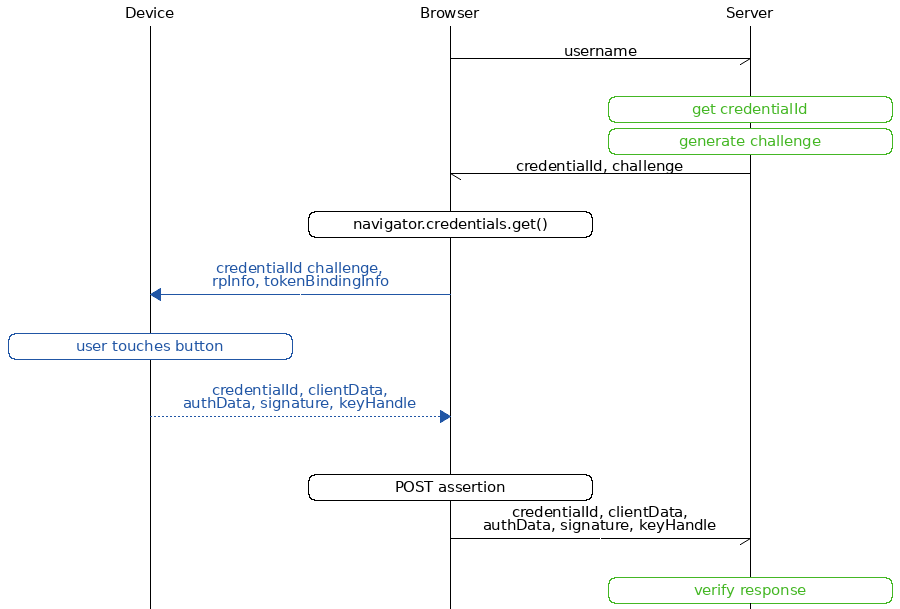
\includegraphics[width=\textwidth]{references/fido_flow_by_yubico.png}
  \caption{FIDO2 authentication sequence diagram [Yubico, 2022]}
  \label{figure_one}
\end{figure}

The CTAPs standardize the communication between a client and a roaming authentication device. The protocols expect the authenticator to obtain evidence of user interaction. Neither the channel between client and the roaming authenticator, nor the transport layer's encryption are currently standardized. The protocol contains the legacy CTAP1 protocol formerly known as the U2F protocol and the current CTAP2 protocol. The CTAP1 authenticators are also called U2F authenticators and the CTAP2 authenticators are also known as WebAuthn or FIDO2 authenticators~\cite{000003,274547,9099190}.

To ensure quality and security, the FIDO Alliance has set up a metadata service that can be inquired to verify the authenticator used for the login. The relying party can check whether the authenticator meets the FIDO Alliance standards and has known vulnerabilities~\cite{9099190}.

\section{Problems of FIDO}
While FIDO2 has advantages over password-based two factor authentication, there are currently some disadvantages and problems that should be considered when evaluating the usability and usefulness of hardware security tokens.

\subsection{Downgrade Attacks}
Besides FIDO, different methods of multifactor authentication exist, like One-Time-Passwords (OTP), confirmation SMS and calls, and the usage of recovery codes~\cite{000004}. Commonly, the user can choose between the configured MFA schemes, but, except for FIDO2, none of the mentioned schemes are secure against real-time phishing. 

While reviewing Alexa's top 100 websites Ulqinaku et al. found out that most of these websites force users to register at least one additional MFA scheme to use FIDO2 in the first place, effectively creating a vulnerability even when FIDO2 is being used because other MFA undermines the security of FIDO2. Only Google, with Google's Advanced Protection, offers a program not relying on weak MFA, but it is opt-in and not actively advertised on the \textit{Google account dashboard}.

The downgrade attack on FIDO2, as shown by Ulqinaku et al., requires that the victim has different and weaker MFAs registered to their account. The goal of the attacker is to display a fake login screen to the user and let the victim choose a weaker MFA scheme, which is vulnerable to real-time phishing. To achieve this goal the attacker has to set up a login page that is comparable to the website from which the attacker wants the login data or sessions. Because the user expects the security key pop-up, the attacker has to display the pop-up on the page as well. The attacker has to know if and when the user has used thier hardware security token to continue the attack. Otherwise, a user could get suspicious. The browser would usually present the pop-up above the webpage containing the domain and ask for the security key, but the WebAuthn standard also contains an API function to detect the presence of an HST without displaying this pop-up. The difference is not easy to spot for a normal user~\cite{274610}.

The authors of the paper suggested a solution for this problem: To disable weaker alternative schemes. They mentioned that this suggestion will come with the problem of non-scalable recovery. This recovery adds significant cost to the service provider and would not scale to millions of users, while also providing an inconvenience for the user. Registering multiple keys can be another solution but may also be costly and create a barrier. Risk-based authentication can be used to determine the authenticity of a recovery process, but recent studies~\cite{10.1145/3372297.3417892} show that these can also be circumvented. Another solution suggested by the authors is to always show the hint when an application tries to access the HST, making it slightly easier for a possible victim to spot the attack.

\subsection{Threats to HST}
The security of FIDO2 is dependent on secure HSTs. Therefore, if the HST is compromised, FIDO2 is not secure anymore. As Pfeffer et al. pointed out, an attacker can get a hold of an access token on the supply chain between a manufacturer and the end-users, either by intercepting the delivery or inserting malicious HST as a manufacturer or a re-seller. An attacker can also buy a genuine token and return malicious HST to the seller through a refund because most sellers will not check if the HST got tampered with~\cite{000007}. Malicious HST can be turned into attack vectors using one or more of the following methods: (1) firmware modification (2) hardware modification. Using firmware modification, an attacker can pre-initialize a token or add malicious code and hardware which exploits e.g. USB interfaces. In the case of hardware modification, an attacker wires the HST up with a wireless transceiver, like a GSM (Global System for Mobile Communications) or a Bluetooth module. Though token replicas are also counted as hardware modification. These replicas are rather easy to create as instructions are publicly available and can be used without expert knowledge. The main goal of both modifications is to extract or fix secrets, e.g. keys or seeds, of the HST so that it has deterministically derived private keys~\cite{272198}. This results in the following attack scenarios.

\paragraph{Run-time secret extraction:}
The run-time secret extraction can be subdivided into in-band and out-of-band attacks. In the in-band case, the HST is modified in a way that it leaks secrets through in-protocol (covert) channels like the signature or other channels used in the transaction. In the out-of-band case, the HST sends the secrets via a different covert channel outside of the protocol like Bluetooth or GSM.

\paragraph{Delivery-time secret extraction:}
The attacker extracts pre-configured keys or seeds through the hardware of software modifications, which allows them to deterministically guess the public-private key pairs used in future authentication.

This described attack is only relevant to HST which are shipped with pre-configured secrets by the manufacturer like YubiKeys. In the case of most HST, and also YubiKeys, these secrets can be changed by the end-user whenever they want with software provided by the vendor.

\paragraph{Secret fixation:}
Another method that allows an attacker to deterministically guess the generated public-private key pair is by pre-loading the secret, also called ``fixing''  it. To permanently fix the secret key, hardware, software or both need to be modified. Also, the attacker can use the vendor's software to achieve thier goal.

\paragraph{Predictable RNG modifcation:}
The \textit{random number generator} (RNG) used for the secure derivation of keys can be manipulated to only create predictable sequences by using hardware and software modifications. The RNG can have unintended weak design, so that no modifications are needed for exploitation. When a weak RNG is used, the attacker can guess the key pair more easily.

\paragraph{Ransom attack:}
Like other ransom attacks, this attack appears as a denial of service attack. The HST is manipulated in such a way that it stops operating after some time, demanding a ransom to resume its work with a threat to delete the stored secrets. This attack has limited viability for FIDO2, since, in most cases, recovery codes are generated upon FIDO2 key registration. This attack is more feasible for hardware wallets (outside of the scope of this paper).

\paragraph{USB pivoting:}
Furthermore, the HST can not only be used to attack authentication flows but also to attack the whole client via the USB interface. If the HST carries malware, it can act as a USB Rubber Ducky (emulate a keyboard) or trigger a buffer overflow.

\paragraph{}
Pfeffer et al. present (already existing) methods to detect a tempered HST.
Modification on hardware or firmware level can be detected with tamper-evident packaging using holographic stickers or other methods. But this is only a low level of protection since holographic stickers are easily replaceable and the attacker can be a manufacturer or re-seller. An HST token can be a single-piece cast, like the Yubikeys, or can be opened. The single-piece cast can be easily inspected but can be broken with household chemicals when the manufacturer foregoes more chemical-resistant plastic. Openable HST can be inspected by users increasing security by visually comparing manufacturer pictures with the present HST. This process has its downsides as it is error-prone and cumbersome. Signals on the printed circuit board (PCB) can be intercepted or manipulated, requiring a secure CPU or other element to shield it. In theory, the key never leaves this secure element and therefore cannot be intercepted. To prevent firmware manipulation, automatic and manual software verification can be used. 

In the case of automatic verification, local and remote validation must be distinguished: Local Validation only validates the integrity by conducting a simple signature check. Remote validation is more sophisticated; the internal status is validated by a third party, making token replicas harder to produce. Both methods need to be visible to the user, otherwise, the user cannot make related trust decisions.
Manual verification can be done by the end-user with HST supporting it, example given YubiKeys, but the corresponding software has to be found, as it is not advertised on the pages of the manufacturer. Moreover, this method is neither explained nor advertised by vendors on delivery, leaving uneducated users in the dark.

A way to prevent attacks on pre-configured secrets is to not ship them at all and let the user generate their secrets themselves. However, the authors state that manual verification and the absence of pre-configured secrets reduce the user-friendliness of HST, which can result in lower market shares~\cite{272198}.

\subsection{Misconceptions}
The study conducted by Lassak et al.~\cite{274547} about misconceptions in FIDO2 Biometric WebAuthn shows that users are not yet educated enough to understand the basic functionality of FIDO2 HSTs. There are, among others, misconceptions about storage location, recovery, and usage of multiple devices. The study was held online with 42 participants from the UK and US. All of them were older than 18. The participants used their android smartphone as the HST.

\paragraph{Storage Location}
The majority of the participants thought that their biometrics were sent in an encrypted fashion to the corresponding service provider. Only 14 participants recognized that the biometrics are stored locally and only 2 recognized that the service provider could not get their biometric data, because it does not have the phone.

Likewise, only 24 participants guessed that their biometric data are not affected in the event of a database breach on the services provider's side.

Overall, only four participants were confident that their biometric data did not leave the phone when they used it for authentication.

\paragraph{Lost HST}
Because the private key used for authentication is stored on a phone, losing the phone can provide an attacker with access to the accounts if they can unlock the secret with a registered method. 39 out of the 42 participants thought that an attacker needs their biometrics for the authentication even though the secret can be unlocked with fallback mechanism likes PIN, pattern, or password, which are easier to obtain for the attacker.

\paragraph{Availability}
If the unlocking of the phone fails via registered biometric data, only five participants were aware that they can unlock the HST with a registered fallback option like PIN, pattern, or password. The other participants stated that they do not have set up backup methods at the service provider or they can contact the service provider to recover their account.

\paragraph{Multiple Devices}
Also, there are misconceptions concerning device sharing. One misconception is that it is possible to use another device (after registering one's biometric data). Only six participants were aware that the public-private key pairs are tied to the authenticating device and that the biometric is only used to decrypt and unlock the private key used for the authentication process. Transferring the private key from one authenticator to another is not intended in the current WebAuthn and FIDO2 specifications. The specifications state, that if this kind of behavior is required a roaming authenticator is needed. However, some service providers also make it possible to register more than one HST for a single account, allowing multiple authenticators to grant access to the account.

\paragraph{Delegating Access}
39 participants answered that it is not possible to grant a trusted person access since the person would not have the required biometric data. The other participants argued that it would be possible to use fallback methods or register the biometric data of the trusted person on the used HST. The latter is right, the token can be unlocked using different biometric data if they are registered on the HST.

\paragraph{}
Lassak et al. conducted another follow-up study with different participants. In this study, the participants were separated into co-design focus groups with the task to come up with notifications that address the following misconceptions. Participants received a short and basic introduction video presenting the mechanics of account creation and authentication, to ensure a general knowledge of FIDO2. Detailed information about FIDO2, especially the underlying public-private key cryptography, was intentionally left out.

In the focus groups, participants stressed the storage location of the used biometric features. Notifications created by the focus groups stated that biometric features never leave the device or that no one has access to the biometric features. The created notifications also promoted the convenience and security of biometric WebAuthn.

They also conducted a third study to review the effectiveness of ideas collected during the second study. Because the key component of the notification created during the second study was the storage location, most of the notifications created for the third study revisited this misconception. Participants received one of the following notifications during account creation: (1) Backed by brand-name, (2) cannot be hacked, (3) biometric data never leaves your device, (4) biometric data only stored on your device, (5) biometric data is never shared with third parties, or (6) a default notification without further information. This study showed that the created notification influenced the perceptions of security and privacy in a positive way.

Based on the collected data the authors stated that services using biometric WebAuthn should inform the user that the biometric data is never sent to nor stored by the website, informing them that the biometric is only used on their device. Information about biometric WebAuthn should also point out its convenience, speed, and ease of use. The authors also mentioned that the mental model of password-based sign-in is responsible for many misconceptions and that it needs more research to create notifications changing this model. They make no specific suggestions on how to overcome the discussed problems~\cite{274547}.

\subsection{Additional Problems} \label{ref1}
Besides the mentioned problems, the FIDO2 standard has other problems which are not related to the implementation. This is highlighted in a study by Lyastani et al.~\cite{9152694}. 

\paragraph{Account Recovery}
A fear the participants of the study had was the loss of the HST, which would have had as a consequence that they would not be able to access their accounts. Currently, other 2FA can be used to allow account access even when an HST fails. Some service provides allow for the setup of additional HST, which is recommended by the FIDO Alliance, or other 2FA schemes, which are vulnerable to e.g. phishing, as shown earlier. Only Google's Advanced Protection Program forces the user to register two HSTs.

This issue is not yet addressed by the FIDO Alliance. The current recommendation is to use additional authenticators. The authors recommend guiding the users in the task of scalable account recovery, but this will not change the fact that account recovery is a serious issue which should be handled by the FIDO instead of a single service provided to create a single way of account recovery. This problem needs attention, especially if FIDO2 should become the only 2FA scheme or even a 1FA, as it can impede future adoption~\cite{9152694}. 

\paragraph{Account Suspension}
The authors themselves raise the concern of how to revoke the HST from an account if the HST of the user is stolen or lost and the user is not able to access the account using other MFA schemes. The FIDO Alliance argues that the risk of such thefts is lower than becoming the victim of a phishing campaign or server breach. The authors are concerned about the effect of FIDO, especially in terms of 1FA, on abusers in intimate partner violence. They are unsure if HST eases or hampers such targeted attacks. Also, the authors state that such behavior is not considered thoroughly enough yet and that users need the possibility to lock their account down without having the HST. They also mentioned that a possible inspiration can be the key revocation in PKI or GPG.

\section{Adoption Barriers}
Farke et al. explored the willingness of users to make use of HST in a study. Since they only had nine participants a general statement cannot be made, but the study can provide insights into reasons that can prevent a wider appeal of HST and FIDO2. The users indicated that they feared losing the HST, the inconvenience of being required to plug in the HST, and the habit of using passwords as adoption barriers.

\paragraph{Convenience}
Three participants stated that the login with an HST requires additional effort and time, making it less convenient than the previously used credentials like username and password. It was also perceived negatively that the setup of the HST took additional time (5 - 10 minutes). This implies that even a short duration of time can reduce the willingness to use HST.

In the study, the workflow was negatively impacted, because using an HST meant that additional steps were required for each login attempt. The click count and the time to log in were mentioned. Also, it was cited that the current implementation of Windows Hello can be a hurdle for adoption because the account selection when using multiple accounts for a single service was not clear. This behavior is implementation-dependent but if a user has to search for the right account in the HST or the authentication device it can prevent the spreading of FIDO2. 

The study also indicated that thought must be given to overcoming old habits and that measures must be taken to widely distribute HST.

\paragraph{}
The authors mention that the participants understand the authentication process using HST and that the authentication time was more of a limiting factor. Compared to the studies presented above, participants in this study received a training session in advance. The difference in speed could be one of the primary adoption barriers for FIDO2 and HST. Also, participants answered that unconscious decisions to use passwords instead of the HST makes it even more difficult to change the mental mindset of the users, in general, to use HST over passwords. Since only the recent version of operating systems and clients were equipped with all WebAuthn features, WebAuthn has the potential to spread better in the future. Since it no longer requires special software or specific knowledge and is thus more accessible to the general public. To overcome the mentioned adoption barriers the authors have the following suggestions: (1) Support for multiple HST (platform and roaming) (2) Requirement of adoption of HST (3) Implementation of FIDO2 in as many as possible services (4) Allow to "remember" the unlock state of HST when using PIN or biometrics~\cite{255646}.

\section{Conclusion}
FIDO2, in combination with hardware security tokens, offers a more secure way of user authentication. This authentication scheme is resistant to all currently used attacks on password flows. It even provides the possibility of single-factor authentication; retiring passwords and their problems. But as we found out, it has its problems and drawbacks. More users would be forced to use FIDO2 if it was more widely implemented on websites, including implementation as the only 2FA option. The argument of the added cost of authentication through expensive tokens can be invalidated with the fact that today around 90 percent of the population already own a mobile phone~\cite{000005}. In our opinion, fundamental user education is needed, but this can be done during the setup of the security tokens on the site of the service providers. More studies addressing the design and content of notification shown to end-user before or during the creation of stronger credentials, like the one conducted by Lassak et al., are needed to better understand how end-users can be recruited to use more secure authentication schemes while also preventing misconceptions from occurring. Hopefully, studies in the future can be used to create a style guide for notifications addressing security, so that the important notification can be standardized. Also, the problems presented in \ref{ref1} need to be more thoroughly considered before FIDO2 has a more sizeable market share to avoid problems with recovery and, especially, to prevent an abuser from accessing the account of a victim.

\section*{Acknowledgments}
We would like to thank our reviewers Alexander, Marc, Oliver, and Yannik for their valuable feedback. We also thank Vincent Drury for being an extremely
supportive point of contact for the creation of this paper.

% Start bibliography
\bibliographystyle{alpha}
\bibliography{literature}

\end{document}
